\section{Introduction}
%
%  Introduction
%


\begin{frame} {Introduction}
  \begin{block}{Part 1 - A Quick Reminder}
    \begin{itemize}
      \item Theoritical Foundations
      \item Fundamental repositories and their role
      \item Installation procedure
    \end{itemize}
  \end{block}
  \begin{block}<2>{Part 2 - A Quick Appetizer}
    \begin{itemize}
      \item Quick start
      \item Software structure
    \end{itemize}
  \end{block}
\end{frame}

\section{Quick start}

\begin{frame}[fragile]{An example with HRP-2}
  \begin{block}{Assumptions}
    \begin{itemize}
      \item OpenHRP 3.0.7 is installed
      \item The Stack of Tasks has been installed thanks to Florent slides with
        \textbf{install\_sot.sh} in the directory:
        \begin{lstlisting}[language=bash,basicstyle=\small,frame=single,showlines=false]    
          /home/user/devel/ros_unstable
        \end{lstlisting}
      \item Your /opt/grx3.0/HRP2LAAS/bin/config.sh is well setup.
    \end{itemize}
  \end{block}
  \begin{block}{The golden commands}
  \begin{lstlisting}[language=bash,basicstyle=\tiny,backgroundcolor=\color{AliceBlue}, frame=single,showlines=false]
    $>roscore
    #Launching HRP2 simulation with OpenHPR
    $>roslaunch hrp2_bringup openhrp_bridge.launch robot_machine_profile:=sim
    $>rosservice call /start_dynamic_graph 
    $>rosrun dynamic_graph_bridge run_command
  \end{lstlisting}
  \end{block}
\end{frame}

\begin{frame}[fragile]{An example}
\begin{block}{Import the graph python module}
  \begin{lstlisting}[language=Python,basicstyle=\small,backgroundcolor=\color{AliceBlue}, frame=single,showlines=false]
[INFO] [WallTime: 1370854858.786392] waiting for service...
Interacting with remote server.
>>> from dynamic_graph.sot.pattern_generator.walking import *
With meta selector
  \end{lstlisting}
\end{block}
\end{frame}


\begin{frame}[fragile]{An example}
\begin{block}{Create the graph}
  \begin{lstlisting}[language=Python,basicstyle=\small,backgroundcolor=\color{AliceBlue}, frame=single,showlines=false]
>>> CreateEverythingForPG(robot,solver)
At this stage
('modelDir: ', '~/devel/ros-unstable/install/share/hrp2-14')
('modelName:', 'HRP2JRLmainsmall.wrl')
('specificitiesPath:', 'HRP2SpecificitiesSmall.xml')
('jointRankPath:', 'HRP2LinkJointRankSmall.xml')
After Task for Right and Left Feet
  \end{lstlisting}
\end{block}
\end{frame}


\begin{frame}[fragile]{An example}
  \begin{block}{Switch to the new graph}       
    \begin{lstlisting}[language=Python,basicstyle=\small,backgroundcolor=\color{AliceBlue}, frame=single,showlines=false]
>>> walkFewSteps(robot)
>>> 
    \end{lstlisting}
  \end{block}
\end{frame}

\section{Software Structure}

\begin{frame}{Software structure - Conceptual view}
  \begin{figure}
    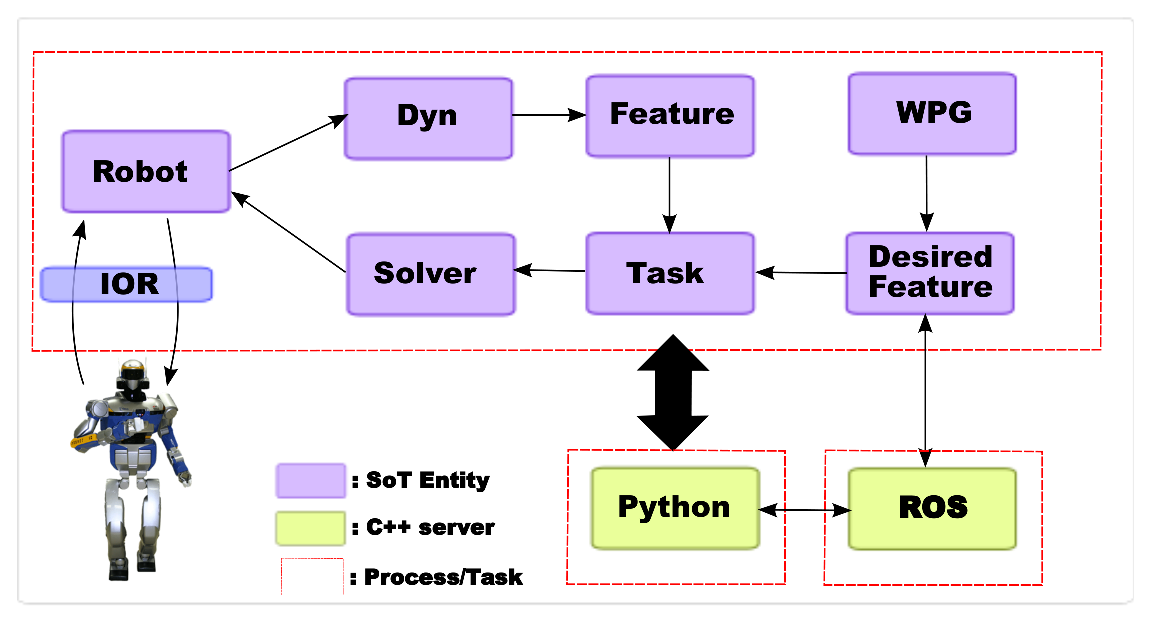
\includegraphics[width=\linewidth]{./figures/Concept-Fig}
  \end{figure}
\end{frame}

\begin{frame}{Software structure - Link with Model}
  \begin{figure}
    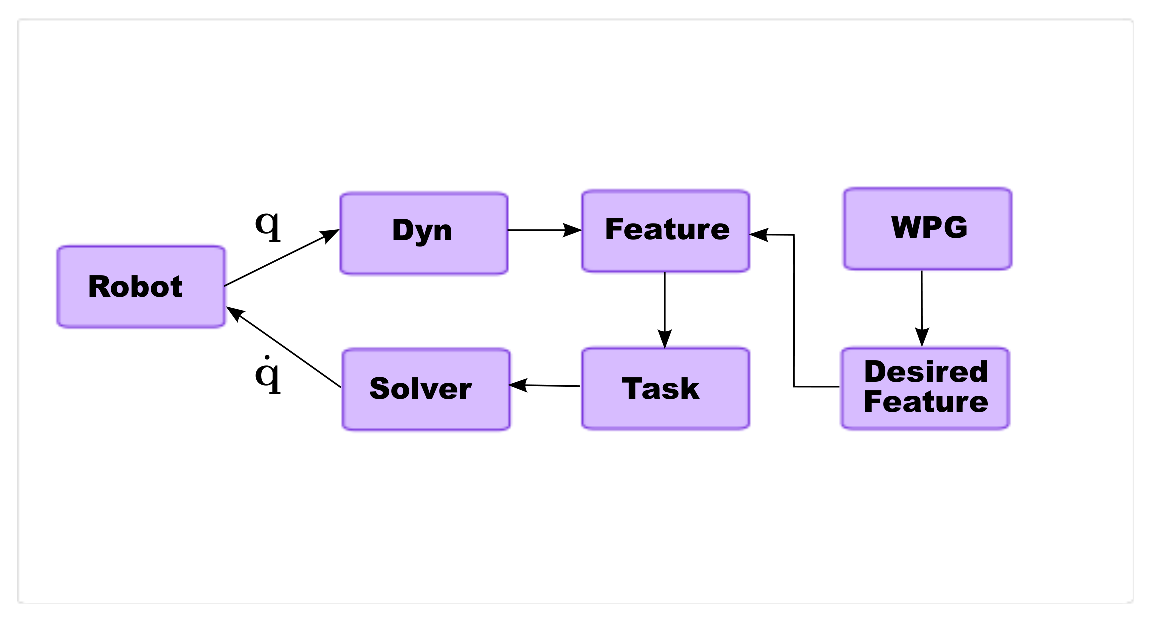
\includegraphics[width=\linewidth]{./figures/Concept-Theory-Fig-Finalv2M5}
  \end{figure}
\end{frame}

%  $$ T ({\bf q}, t) = \left(\begin{array}{cc} {\bf t} (M^{* -1}(t) M ({\bf q})) \\ u_{\theta} (R^{* -1}(t) R ({\bf q})) \end{array}\right) $$
    
% $ J=  \frac{\partial T}{\partial {\bf q}}$
 
% $\dot{T} = - \lambda T

% $\dot{T} = - \lambda T - \frac{\partial T}{\partial t} $

% $\dot{{\bf q}} \triangleq& -J ^{+} (\lambda T + \frac{\partial T}{\partial t} $

\begin{frame}{Software structure - Link with Model}
  \begin{figure}
    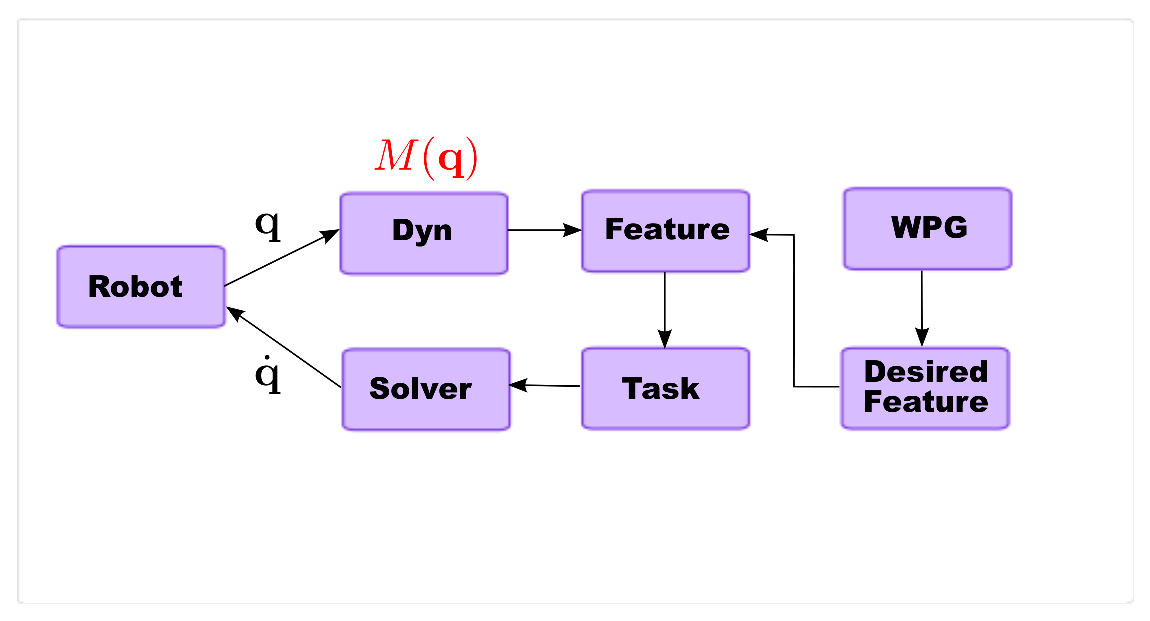
\includegraphics[width=\linewidth]{./figures/Concept-Theory-Fig-Finalv2M4}
  \end{figure}
\end{frame}

\begin{frame}{Software structure - Link with Model}
  \begin{figure}
    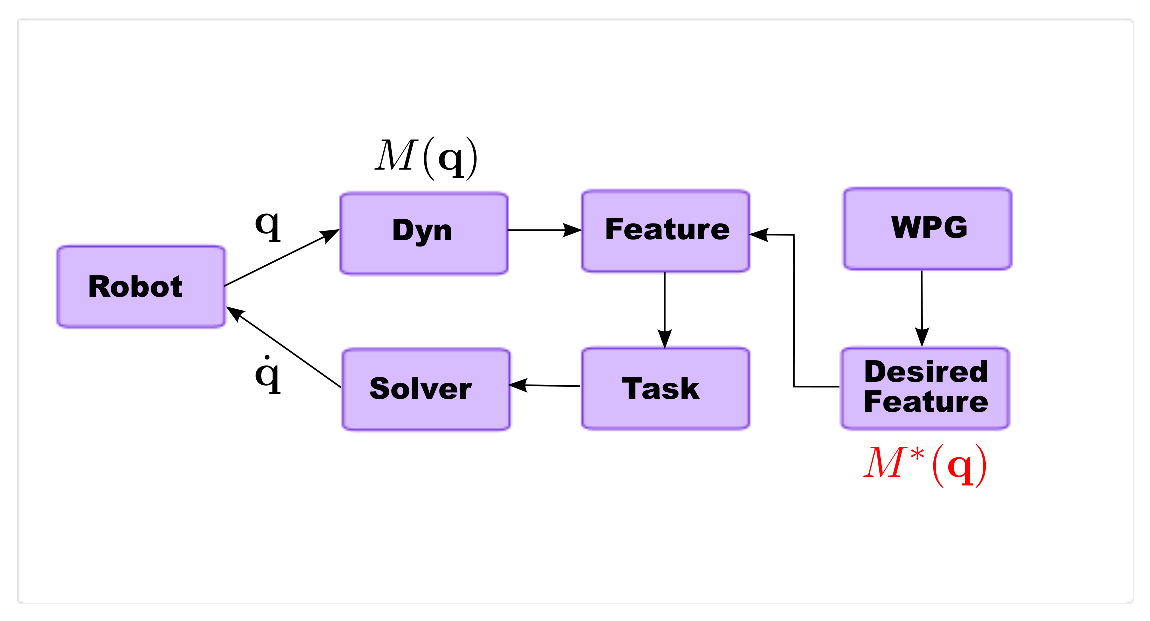
\includegraphics[width=\linewidth]{./figures/Concept-Theory-Fig-Finalv2M3}
  \end{figure}
\end{frame}

\begin{frame}{Software structure - Link with Model}
  \begin{figure}
    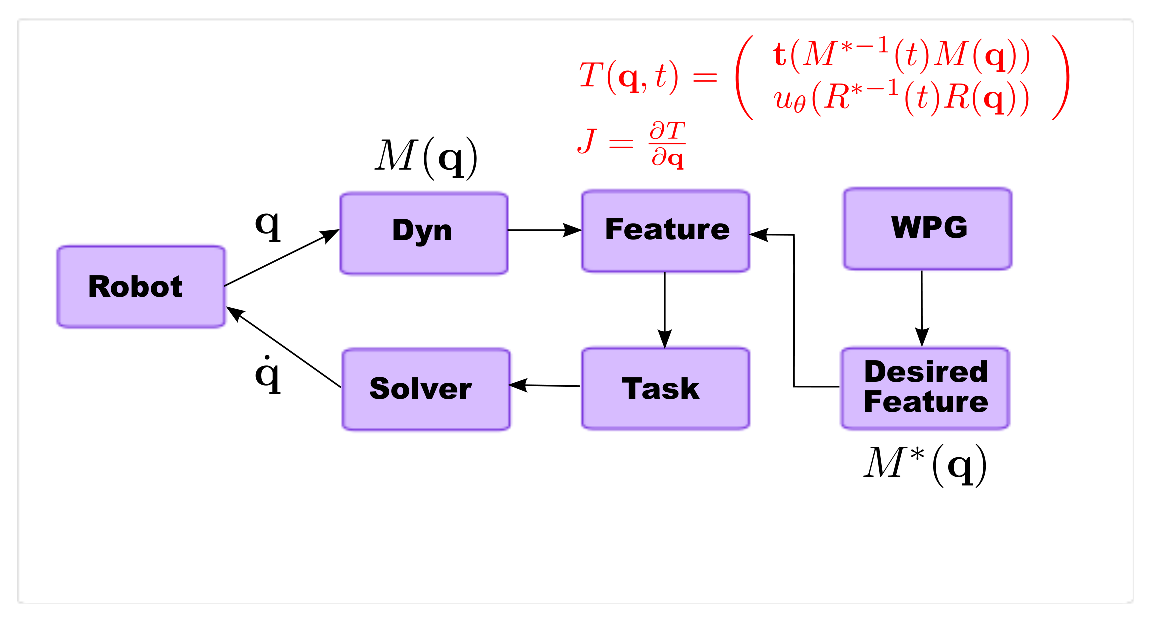
\includegraphics[width=\linewidth]{./figures/Concept-Theory-Fig-Finalv2M2}
  \end{figure}
\end{frame}

\begin{frame}{Software structure - Link with Model}
  \begin{figure}
    \includegraphics[width=\linewidth]{./figures/Concept-Theory-Fig-Finalv2M1}
  \end{figure}
\end{frame}

\begin{frame}{Software structure - Link with Model}
  \begin{figure}
    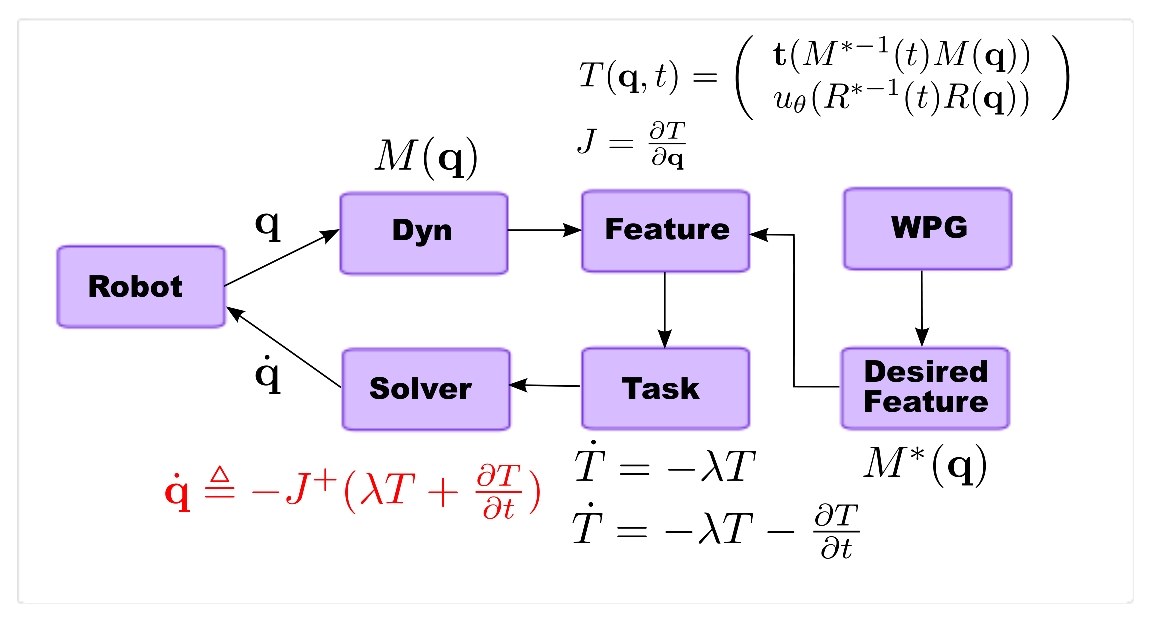
\includegraphics[width=\linewidth]{./figures/Concept-Theory-Fig-Finalv2}
  \end{figure}
\end{frame}

\begin{frame}{Software structure - Repositories}
  \begin{figure}
    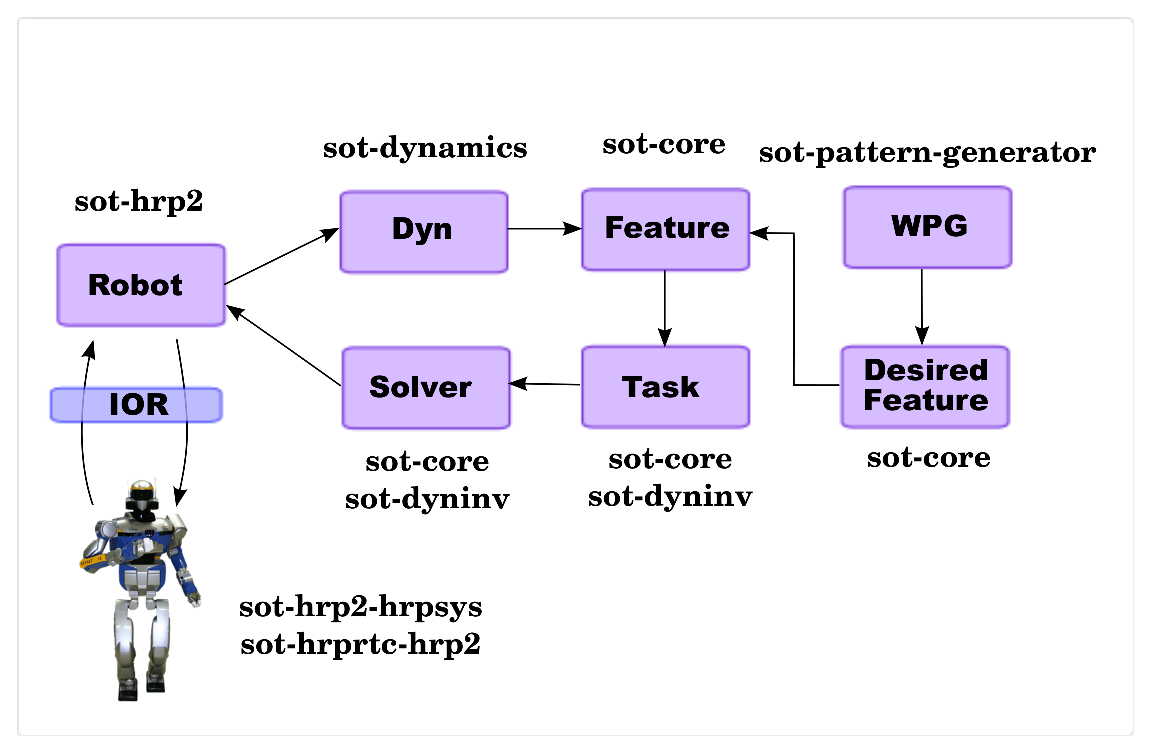
\includegraphics[width=\linewidth]{./figures/Concept-Software-Fig}
  \end{figure}
\end{frame}

